% TeXplates/Mathematics.tex
% v0.8.0
% https://github.com/HoyanMok/TeXplates
\documentclass[openany, a5paper]{book} 
% \documentclass{ctexbook} 如果用中文
% \documentclass[10pt,a4paper]{ctexart}  字体大小和纸张大小,默认分别为10pt和letterpaper
% 五号 = 10.5pt,小四=12pt,四号=14pt
% 其他可选参量如twocolumn, 两行排版



\usepackage{../TeXplatesMathematics}
\addbibresource{FunctionalAnalysis.bib} % 把这里改成实际的文件名
% \usepackage{fontspec}
% \defaultfontfeatures{Ligatures=TeX}

% 文章标题页信息:
\title{Functional Analysis}
\author{Hoyan Mok}
\date{\today} % 自动生成日期
\titlepic{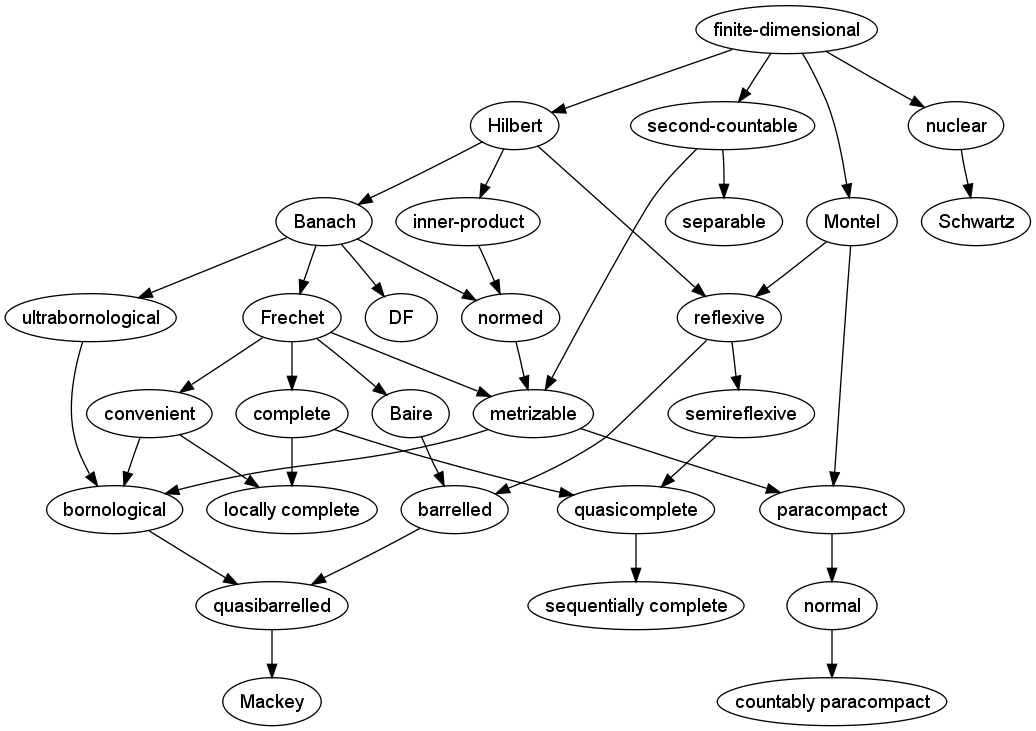
\includegraphics[width=.8\textwidth]{topvs.png}}

\begin{document}
\pagenumbering{Alph}
\maketitle % 打印标题
\frontmatter
\chapter{Preface}
Preface.

\tableofcontents

\mainmatter
\chapter{Topological Vector Spaces}

\section{Topological Vector Spaces}

If not specified, $\mathbb K$ is either $\mathbb R$ or $\mathbb C$, $V$ is a vector space over $\mathbb K$.

\begin{definition}[Topological Vector Space]%
	\label{def: topological vector space}
	A \indexbf{topological vector space} is a vector space $V$ over field $\mathbb K$ ($\mathbb K = \mathbb R \vee \mathbb K = \mathbb C$) s.t.\ 
	the vector addition $+\colon V \times V \to V$ and the scalar multiplication $\cdot \colon \mathbb K \times V \to V$ are both continuous.
\end{definition}


\begin{definition}[Balanced set]%
	\label{def: balanced set}
	A subset $C$ of  $V$ over $\mathbb K$ is \indexbf{balanced} if $\forall \lambda \in \mathbb K$,  $\forall x \in C$, if $|\lambda| \leq 1$, then $\lambda x \in C$.
\end{definition}
It means that, if $x \in C$, the disk with $x$ on its boundary and centered at $0$ is also contained in $C$.


\begin{definition}[Locally convexity]%
	\label{def: locally convexity}
	A topological vector space $V$ is \indexbf{locally convex} if there exists a local base of balanced, convex sets at $0$.
\end{definition}


\chapter{Normed and Banach Spaces}

\chapter{Inner Product and Hilbert Spaces}

\chapter{Linear Operators}




\chapter{Duality and Hahn-Banach Theorem}

\section{Sublinear Functionals}


\begin{definition}[Sublinear functional]
	Let $V$ be a vector space over $\mathbb K$ ($\mathbb K = \mathbb R \vee \mathbb K = \mathbb C$).
	A \indexbf{sublinear functional} on $V$ is a function $p\colon V \to \mathbb R$ s.t.\
	\begin{enumerate}
		\item  $\forall v \in V$, $\forall \lambda \in \mathbb R$, if $\lambda \geq 0$, then $p(\lambda v) = \lambda p(v)$
		(\indexbf{non-negative homogeneity} or \indexbf{positive homogeneity});
		\item  $p(v + w) \leq p(v) + p(w)$ for all $v, w \in V$ (\indexbf{subadditivity} or \indexbf{triangle inequality}).
	\end{enumerate}
\end{definition}


\begin{definition}[Semi-norm]%
	\label{def: semi-norm}
	A \indexbf{semi-norm} on a vector space $V$ over $\mathbb K$ 
		($\mathbb K = \mathbb R \vee \mathbb K = \mathbb C$) 
		is a function $p\colon V \to \mathbb R$ s.t.\ 
	\begin{enumerate}
		\item  $\forall v \in V$, $\forall \lambda \in \mathbb K$, $p(\lambda v) = |\lambda| p(v)$
		(\indexbf{absolute homogeneity});
		\item  $p(v + w) \leq p(v) + p(w)$ for all $v, w \in V$ (\indexbf{subadditivity}).
	\end{enumerate}
\end{definition}

The definition implies that a semi-norm is also non-negative ($p(v) \geq 0$).

By comparing definition, we can tell that a semi-norm is a sublinear functional, and a norm is a semi-norm with $p(v) > 0$ for non-zero $v$.

\section{The Hahn-Banach Theorem}

\begin{definition}[Extension]
	An \indexbf{extension} of a linear functional $f_W\colon W \to \mathbb K$ on a subspace $W$ of a vector space $V$ over $\mathbb K$ is a linear functional $f\colon V \to \mathbb K$ s.t.\ 
	\begin{equation*}
		\forall w \in W, \;
		f(w) = f_W(w).
	\end{equation*}
\end{definition}


\begin{theorem}[Hahn-Banach]%
	\label{thm: Hahn-Banach}\index{Hahn-Banach theorem}
	Let $V$ be a vector space over $\mathbb K$ ($\mathbb K = \mathbb R \vee \mathbb K = \mathbb C$).
	$p\colon V \to \mathbb R$ is a seminorm.
	$W \subset V$ is a subspace of $V$.

	If $f_W\colon W \to \mathbb K$ is a linear functional s.t.\ 
	\begin{equation*}
		\forall w \in W, \;
		|f_W(w)| \leq p(w),
	\end{equation*}
	then there exists an extension $f \colon V \to \mathbb K$ s.t.\ 
	\begin{equation*}
		\forall v \in V, \;
		|f(v)| \leq p(v).
	\end{equation*}
\end{theorem}

\chapter{Linear Operators on Hilbert Spaces}

\chapter{Compact Operators}

\chapter{Integral and Differential Equations}

\appendix
\renewcommand{\theequation}{\Alph{chapter}-\arabic{equation}}
\chapter{Appendix}

\backmatter
\nocite{*} % 这个表示列出所有没有在文中被引用的参考文献
\printbibliography[heading=bibliography, title={Bibliography}]

\indexprologue{Here listed the important symbols used in this notes.}
\printindex[symbol]

\printindex

\end{document}